\section{Compositional Embeddings} \label{sec:lang}

After looking back at the existing embedding techniques, this section shows that
compositional programming enables a new form of DSL embedding called a
\emph{compositional embedding}. Compositional programming is a statically typed
modular programming paradigm implemented by the CP language. For the details of
the semantics of CP, we refer the reader to work by
\citet{zhang2021compositional}. We have reimplemented CP as an in-browser
interpreter, which can be directly run on a serverless web page. There are some
small syntactic differences between our implementation and the original work,
which we point out when necessary. Additionally, our implementation uses the
call-by-need evaluation strategy, which optimizes the original call-by-name one.

Here, we only introduce the necessary language features of CP to illustrate
compositional embeddings. With compositional embeddings, we can get many of the
benefits of both shallow and deep embeddings without most of the drawbacks. We
revisit the challenges illustrated in \autoref{sec:embed} using our approach in
this section. A detailed comparison between compositional embeddings and various
existing forms of embeddings, including shallow, deep, hybrid, and polymorphic
embeddings, is presented at the end of this section.

\subsection{Initial System, Revisited: Compositional Interfaces and Traits}

As before, we start with an initial language interface inspired by
\citet{hudak1998modular} and an abstract interpretation that calculates the
syntactic size of a region:

\begin{lstlisting}
type Vector = { x: Double; y: Double };

type HudakSig<Region> = {
  Circle:    Double -> Region;
  Outside:   Region -> Region;
  Union:     Region -> Region -> Region;
  Intersect: Region -> Region -> Region;
  Translate: Vector -> Region -> Region;
};

type Size = { size: Int };
sz = trait implements HudakSig<Size> => {
  (Circle      _).size = 1;
  (Outside     a).size = a.size + 1;
  (Union     a b).size = a.size + b.size + 1;
  (Intersect a b).size = a.size + b.size + 1;
  (Translate _ a).size = a.size + 1;
};
\end{lstlisting}

\noindent
Since CP is also statically typed, a \emph{compositional interface}
(\lstinline{HudakSig}) serves as the specification of the DSL syntax, playing a
similar role to algebraic data types in the deep embedding. The type parameter
\lstinline{Region} is called the \emph{sort} of the interface
\lstinline{HudakSig}. Sorts can be instantiated with different concrete types
that represent different semantic domains. Every constructor, which is
capitalized, must return a sort. Compositional interfaces are implemented by
\emph{traits}~\citep{ducasse2006traits,bi2018typed}, which serve as the unit of
code reuse in CP. Traits play a similar role to classes in traditional
object-oriented languages and are used to provide implementations for
interpretations of the region DSL. To implement the abstract interpretation of
the DSL, we first define the semantic domain type \lstinline{Size}. Then we
define a trait that implements \lstinline{HudakSig<Size>}. In the body of the
trait, we use \emph{method patterns}, such as \lstinline{(Circle _).size = 1},
to define the implementation. The method patterns used in the trait body allow
us to define interpretations that look very much like the corresponding
definition of \lstinline{size} by pattern matching in Haskell in
\autoref{fig:pattern}.

\subsection{Linguistic Reuse and Meta-Language Optimizations} \label{sec:sharing}

The example of horizontally aligned circles in \autoref{sec:meta} can be
translated to CP as:

\begin{lstlisting}
sharing Region = trait [self: HudakSig<Region>] => open self in {
  circles = letrec go (n: Int) (offset: Double): Region =
              if n == 0 then Circle 1.0
              else let shared = go (n-1) (offset/2.0)
                   in Union (Translate { x = -offset; y = 0.0 } shared)
                            (Translate { x =  offset; y = 0.0 } shared)
            in go 20 (pow 2.0 18);
};
\end{lstlisting}

\noindent
Since the region DSL can have multiple interpretations, \lstinline{circles}
should be oblivious of any concrete interpretation but only refer to the
language interface. To achieve this, we use \emph{self-type annotations}. The
trait \lstinline{sharing} is parametrized by a type parameter \lstinline{Region}
and annotated with a self-type \lstinline{HudakSig<Region>}. Like Scala traits,
CP traits can be annotated with self-types to express abstract dependencies.
This serves as an elegant way to inject region constructors. All of the
constructors formerly declared in the interface are available through
self-references, for instance, \lstinline{open self in ... Circle 1.0}. These
constructors are \emph{virtual}~\citep{madsen1989virtual,ernst2006virtual}: they
are not attached to a specific implementation.

With the self-type dependency on \lstinline{HudakSig<Region>}, the static type
checker of CP rejects a direct instantiation like \lstinline{new sharing @Size}
(\lstinline{@} is the prefix for a type argument). Instead, we need to compose
\lstinline{sharing} with a trait implementing \lstinline{HudakSig<Size>}, using
a \emph{merge operator}~\citep{dunfield2014elaborating}:

\begin{lstlisting}
test = new sharing @Size , sz;            -- test = new ((sharing @Size) , sz);
test.circles.size            -- Above is equivalent with redundant parentheses.
\end{lstlisting}

\noindent
The merge of the two traits (\lstinline{sharing @Size} and \lstinline{sz}) is
still a trait. With self-type dependencies satisfied, the merged trait can be
instantiated successfully, and we can call its method. According to call-by-need
evaluation, the result of \lstinline{shared} is stored for subsequent use once
evaluated. Thanks to the linguistic reuse of the host-language \lstinline{let}
expressions and their optimizations, evaluating \lstinline{circles.size} is able
to exploit sharing and terminates almost immediately. This is similar to the
Haskell approach in \autoref{sec:meta} using shallow embeddings.

\subsection{Adding New Language Constructs}\label{sec:syntax}

In compositional embeddings, language constructs can be modularly added. We
first create a new language interface inspired by \citet{hofer2008polymorphic}
and then define a trait implementing it:

\noindent
\begin{minipage}{.45\textwidth}
\begin{lstlisting}
type HoferSig<Region> = {
  Univ: Region;
  Empty: Region;
  Scale: Vector -> Region
                -> Region;
};
\end{lstlisting}
\end{minipage}%
\begin{minipage}{.55\textwidth}
\begin{lstlisting}[showlines]
sz' = trait implements HoferSig<Size> => {
  (Univ     ).size = 1;
  (Empty    ).size = 1;
  (Scale _ a).size = a.size + 1;
};
 
\end{lstlisting}
\end{minipage}

\noindent
To compose multiple interfaces, we use \emph{intersection types}. To illustrate
this, we create a repository of shapes that make use of language constructs from
both interfaces:

\begin{lstlisting}
type RegionSig<Region> = HudakSig<Region> & HoferSig<Region>;
repo Region = trait [self: RegionSig<Region>] => open self in {
  ellipse = Scale { x = 4.0; y = 8.0 } (Circle 1.0);
  universal = Union (Outside Empty) (Circle 1.0);
};
\end{lstlisting}

\noindent
\lstinline{RegionSig} is an intersection type combining the two interfaces into
one. The definition of \lstinline{repo} is similar to the definition of
\lstinline{sharing} in \autoref{sec:sharing}. It defines an ellipse, by using
the \lstinline{Scale} constructor from \lstinline{HoferSig} and the
\lstinline{Circle} constructor from \lstinline{HudakSig}. Similarly, it defines
an essentially universal region by using constructors from both signatures.

\subsection{Adding New Interpretations} \label{sec:semantics}

Besides language constructs, it is also trivial to add new semantic
interpretations in compositional embeddings. Just like creating a new
interpretation function in deep embeddings, we only need to define a new trait
implementing a compositional interface:

\begin{lstlisting}
type Eval = { contains: Vector -> Bool };
eval = trait implements RegionSig<Eval> => {
  (Circle         r).contains p = pow p.x 2 + pow p.y 2 <= pow r 2;
  (Outside        a).contains p = not (a.contains p);
  (Union        a b).contains p = a.contains p || b.contains p;
  (Intersect    a b).contains p = a.contains p && b.contains p;
  (Translate {..} a).contains p = a.contains { x = p.x - x; y = p.y - y };
  (Univ            ).contains _ = true;
  (Empty           ).contains _ = false;
  (Scale     {..} a).contains p = a.contains { x = p.x / x; y = p.y / y };
};
\end{lstlisting}

\noindent
Similarly to Haskell, CP supports record wildcards \lstinline|{..}|, which bring
record fields into scope. We instantiate the sort with a function checking if a
point resides in a region.

\paragraph{Composing multiple interpretations.}
Now that we have multiple interpretations, we use \emph{nested trait composition},
provided by the merge operator, to compose all interpretations:

\begin{lstlisting}
shapes = new repo @(Eval&Size) , eval , sz , sz';  -- nested trait composition

"The elliptical region of size " ++ toString shapes.ellipse.size ++
(if shapes.ellipse.contains { x = 0.0; y = 0.0 }
 then " contains " else " does not contain ") ++ "the origin."
--> "The elliptical region of size 2 contains the origin."
\end{lstlisting}

\begin{figure}
  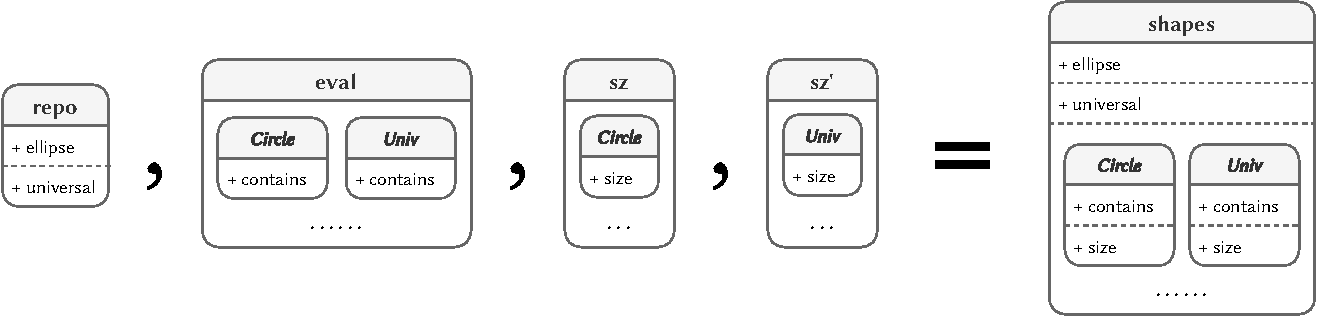
\includegraphics[width=\textwidth]{merge.pdf}
  \caption{A visualization of nested trait composition.} \label{fig:compose}
\end{figure}

\noindent
We provide the final semantic domain (\lstinline{Eval&Size}), as the type
argument, for the trait \lstinline{repo} and merge it with three other modularly
defined traits. The trait composition is called
\emph{nested}~\citep{bi2018essence} because not only different sets of
constructors, but also different semantics nested in the same constructor are
merged. In our case, both interpretations are available under the two sets of
language constructs after nested composition, as visualized in
\autoref{fig:compose}. Here, the language constructs and their semantics form a
two-level hierarchy of traits. Such composition of whole hierarchies can be
traced back to \emph{family polymorphism}~\citep{ernst2001family}. With this
powerful mechanism of nested composition, we can easily develop highly modular
\emph{product lines}~\citep{apel2013feature} of DSLs, where DSL features can be
composed \emph{à la carte}.

\subsection{Dependency Injection and Domain-Specific Optimizations} \label{sec:deps}

Now we illustrate CP's support for \emph{modular dependent interpretations}. We
skip the simpler example with \lstinline{text} and focus on the more interesting
example with \lstinline{isUniv} and \lstinline{isEmpty}. Similarly to the deep
embedding in Haskell in \autoref{sec:transform}, we define two compositional
traits \lstinline{chkUniv} and \lstinline{chkEmpty}:

\begin{lstlisting}
type IsUniv  = { isUniv:  Bool };
type IsEmpty = { isEmpty: Bool };

chkUniv = trait implements RegionSig<IsEmpty => IsUniv> => {
  (Univ         ).isUniv = true;
  (Outside     a).isUniv = a.isEmpty;
  (Union     a b).isUniv = a.isUniv || b.isUniv;
  (Intersect a b).isUniv = a.isUniv && b.isUniv;
  (Translate _ a).isUniv = a.isUniv;
  (Scale     _ a).isUniv = a.isUniv;
                _.isUniv = false;
};

chkEmpty = trait implements RegionSig<IsUniv => IsEmpty> => {
  (Empty        ).isEmpty = true;
  (Outside     a).isEmpty = a.isUniv;
  (Union     a b).isEmpty = a.isEmpty && b.isEmpty;
  (Intersect a b).isEmpty = a.isEmpty || b.isEmpty;
  (Translate _ a).isEmpty = a.isEmpty;
  (Scale     _ a).isEmpty = a.isEmpty;
                _.isEmpty = false;
};
\end{lstlisting}

\noindent
The first thing to note is that the sort of \lstinline{RegionSig} is
instantiated with two types separated by a fat arrow (\lstinline{=>}). This is
how we \emph{refine} interface types for dependency injection. For example,
\lstinline{chkUniv} does not implement \lstinline{RegionSig<IsEmpty>}, but we
assume the latter is available. The static type checker of CP guarantees that
\lstinline{chkUniv} is later merged with another trait that implements
\lstinline{RegionSig<IsEmpty>}. That is why we can safely use
\lstinline{a.isEmpty} when implementing \lstinline{(Outside a).isUniv}. The
second trait \lstinline{chkEmpty} is just the dual of \lstinline{chkUniv}. It is
hard to define such interpretations modularly in traditional approaches because
they are dependent, but we make them compositional via dependency injection.
Lastly, \lstinline{_.isUniv} and \lstinline{_.isEmpty} are \emph{default
patterns}, which compensate for the remaining constructors declared in the
interface. For example, \lstinline{_.isUniv = false} implies
\lstinline{Empty.isUniv = false} and \lstinline{Circle.isUniv = false}. Note
that in CP, for modularity, patterns are \emph{unordered}, unlike functional
languages like Haskell or ML. Therefore, default patterns are local to the
traits where they are used. These patterns can be understood as a concise way to
fill the missing cases in the local trait. 

Another thing worth noting is that dependency injection in compositional
embeddings is more modular than direct dependencies in deep embeddings because
the former does not refer to concrete implementations. For example, in the
compositional embedding above, \lstinline{chkUniv} only requires that the
dependent trait should implement the interface \lstinline{RegionSig<IsEmpty>}.
However, in the deep embedding (see \autoref{sec:mutual}), \lstinline{isUniv}
depends on the specific \lstinline{isEmpty} implementation.

\paragraph{Delegated method patterns.}
In some complicated transformations, nested pattern matching is required to
inspect smaller constructs. Nested pattern matching is not directly supported in
CP yet. However, there is a simple transformation that we can do whenever we
would like to have nested patterns:  we can delegate the inner tasks to other
methods whereby only top-level patterns are needed. We call such a technique
\emph{delegated method patterns}.

Concerning the nested pattern matching in \autoref{sec:nested}, we can implement
it with two mutually dependent methods. Since delegated method patterns are not
reused, the two methods are defined together for the sake of simplicity (but can
always be separated into two traits):

\begin{lstlisting}
type Eliminate Region = { eliminate: Region; delOutside: Region };

elim Region = trait [fself: RegionSig<Region>]
              implements RegionSig<Region=>Eliminate Region> => open fself in {
  (Outside     a).eliminate = a.delOutside;
  (Union     a b).eliminate = Union a.eliminate b.eliminate;
  (Intersect a b).eliminate = Intersect a.eliminate b.eliminate;
  (Translate v a).eliminate = Translate v a.eliminate;
  (Scale     v a).eliminate = Scale v a.eliminate;
           [self].eliminate = self;

  -- delegated method patterns:
  (Outside a).delOutside = a.eliminate;
       [self].delOutside = Outside self.eliminate;
};
\end{lstlisting}

\noindent The translation from nested pattern matching to delegated method
patterns is straightforward. Our code lifts nested patterns
(\lstinline{Outside (Outside a)}) to top-level delegated patterns. In this way,
we do not change the underlying algorithm at all. This is in contrast with
approaches like tagless-final embeddings that, as discussed in
\autoref{sec:transform}, seem unable to directly support nested patterns,
requiring different algorithms to achieve the same goal. Though our approach is
not as convenient as deep embeddings, it is noteworthy that we can just write
the original algorithm \emph{modularly}.

If we add new language constructs in the future, it is easy to augment the
traits with more top-level patterns, but extending nested patterns is difficult
because there is no name to denote the \emph{extension point}. With delegated
method patterns, the method name \lstinline{delOutside} offers an extension
point for additional cases in the nested pattern matching. For instance, if we
wish for an extension supporting a new kind of region and a special case for
eliminating a region outside this kind of region
(\lstinline{eliminate (Outside (SomeRegion params))}), we can have a trait with
a method pattern of the following form, modularly defined in another trait:

\begin{lstlisting}
(SomeRegion params).delOutside = ...
\end{lstlisting}

\noindent
Although we believe that the design of CP can be improved to better support
similar logic to nested patterns, there are important differences between
traditional (closed) forms of pattern matching and open pattern
matching~\citep{zhang2020castor}. For instance, patterns in CP are unordered for
compositionality, but the order of patterns matters in conventional pattern
matching. Thus the design of improved language support for nested patterns in
CP, which could make the use of delegated method patterns more convenient,
requires further research and is left for future work.

\paragraph{Linguistic reuse after transformations.}
Before finishing the discussion of modular transformations, let us revisit CP's
support for linguistic reuse: can we still have meta-language optimizations for
free after complicated transformations? The answer is yes. To demonstrate this
point, we can modify the definition of \lstinline{circles} in
\autoref{sec:sharing} to have an inefficient
\lstinline{Outside (Outside (Circle 1.0))}. As usual, we compose all the
necessary traits together to make sure no dependencies are missing:

\begin{lstlisting}
test' = new sharing' @(Size & Eliminate Size) , sz , sz' , elim @Size;
test'.circles.eliminate.size
\end{lstlisting}

\noindent
The evaluation terminates as quickly as before, meaning that meta-language
optimizations are still performed even after a transformation.

We should remark that there are limits to the form of implicit sharing (and
linguistic reuse) that shallow embeddings or compositional embeddings provide.
For both shallow and compositional embeddings, implicit sharing will not work if
the interpretation is a function, such as \lstinline{contains}. In such cases,
the sharing is still lost. Nevertheless, implicit sharing is an important
feature that is often exploited in shallow DSLs. With compositional embeddings,
we can take this idea further and make it work even after some transformations
and optimizations have been applied. Moreover, it is also possible to adopt
solutions with explicit sharing by modeling a \lstinline{Let} construct in the
DSL.

\subsection{A Detailed Comparison between Different Embedding Approaches} \label{sec:comparison}

\newcommand\super[1]{\makebox[0pt]{$\;^#1$}}

\begin{table}
\caption{A detailed comparison between different embedding approaches.} \label{tab:comparison}
\centering
\begin{tabular}{*{6}{c}}
\toprule
                                       &\textsc{Shallow}&    \textsc{Deep}   &    \textsc{Hybrid} &    \textsc{Poly.}  &    \textsc{Comp.}  \\
\midrule \midrule
Transcoding free                       &    \CIRCLE     &    \CIRCLE         &    \Circle         &    \CIRCLE         &    \CIRCLE         \\
Linguistic reuse                       &    \CIRCLE     &    \Circle         &    \CIRCLE         &    \CIRCLE         &    \CIRCLE         \\
Language construct extensibility       &    \CIRCLE     &    \Circle         &\LEFTcircle\super{1}&    \CIRCLE         &    \CIRCLE         \\
Interpretation extensibility           &    \Circle     &    \CIRCLE         &    \CIRCLE         &    \CIRCLE         &    \CIRCLE         \\
Transformations and optimizations      &    \Circle     &    \CIRCLE         &    \CIRCLE         &\LEFTcircle\super{2}&\LEFTcircle\super{2}\\
Linguistic reuse after transformations &    \em n/a     &    \Circle         &    \Circle         &    \CIRCLE         &    \CIRCLE         \\
Modular dependencies                   &    \Circle     &\LEFTcircle\super{3}&\LEFTcircle\super{3}&    \Circle         &    \CIRCLE         \\
Nested pattern matching                &    \Circle     &    \CIRCLE         &    \CIRCLE         &    \Circle         &\LEFTcircle\super{4}\\
\bottomrule
\end{tabular}
\vskip 1ex
{\footnotesize
  $^1$ The extensibility of language constructs is limited or precludes exhaustive pattern matching.\\
  $^2$ Transformations require some ingenuity and are sometimes awkward to write.\\
  $^3$ Dependencies do not require code duplication but still refer to concrete implementations.\\
  $^4$ Nested pattern matching is implemented as delegated method patterns.\\
}
\end{table}

\noindent
In \autoref{tab:comparison}, we compare existing embedding approaches in the
literature with compositional embeddings. Shallow and deep embeddings have been
discussed in detail in \autoref{sec:embed}, and the table summarizes the points
that we have made. Hybrid
approaches~\citep{rompf2012scala,svenningsson2015combining,jovanovic2014yinyang}
employ both embeddings together. However, transcoding from shallow to deep is
generally needed, as both shallow and deep implementations must coexist side by
side. There is a clear boundary between the two parts: linguistic reuse is
available only in the shallow part, while complex transformations are available
only in the deep part. Therefore, it is still hard to exploit host-language
features after transformations. In work by
\citeauthor{svenningsson2015combining}, we cannot add more constructs to the
deeply embedded AST but can only extend shallowly embedded syntactic sugar. In
Scala, if \emph{open} case classes~\citep{emir2007matching} are used for deep
embeddings, ASTs are also extensible but do not ensure the exhaustiveness of
pattern matching. Compositional embeddings offer a unified approach directly
capable of all these functionalities.

\paragraph{Non-modular dependencies in modular embeddings.}
Polymorphic embeddings~\citep{hofer2008polymorphic}, tagless-final
embeddings~\citep{carette2009finally,kiselyov2010typed}, and object
algebras~\citep{oliveira2012extensibility} (denoted as \textsc{Poly.} in the
table) also provide a unified encoding where most advantages of shallow and deep
embeddings are available. However, they cannot deal with dependencies modularly.
Let us take tagless-final embeddings for example, which can also be implemented
in Haskell. We refer curious readers to \autoref{sec:tagless} for the complete
code.

In the tagless-final embedding, region constructors are defined in a type class
instead of a closed algebraic data type, and \lstinline{Size} can be modularly
defined as an instance of the type class since it has no dependency:

\noindent
\begin{minipage}{0.48\textwidth}
\begin{lstlisting}[language=Haskell,deletekeywords={union,intersect}]

class RegionHudak repr where
  circle    :: Double -> repr
  outside   :: repr -> repr
  union     :: repr -> repr -> repr
  intersect :: repr -> repr -> repr
  translate :: Vector -> repr -> repr
\end{lstlisting}
\end{minipage}%
\begin{minipage}{0.52\textwidth}
\begin{lstlisting}[language=Haskell,deletekeywords={union,intersect}]
newtype Size = S { size :: Int }
instance RegionHudak Size where
  circle      _ = S 1
  outside     a = S $ a.size + 1
  union     a b = S $ a.size + b.size + 1
  intersect a b = S $ a.size + b.size + 1
  translate _ a = S $ a.size + 1
\end{lstlisting}
\end{minipage}

\noindent
But how about the textual representation? As a first try, we might write:

\begin{lstlisting}[language=Haskell]
newtype Text = T { text :: String }
instance RegionHudak Text where
  circle  r = T { text = "circular region of radius " ++ show r }
  outside a = T { text = "outside a region of size " ++ show a.size }
  ......
\end{lstlisting}

\noindent
Unfortunately, we will get a type error concerning \lstinline{a.size} because
\lstinline{a} has type \lstinline{Text} and thus does not contain a field named
\lstinline{size}. Once we need operations that have some dependencies on other
operations, we get into trouble!

A simple workaround is to pack the two operations together and duplicate the
code of size calculation. We have already described this approach for shallow
embeddings in \autoref{sec:transform}, and the same workaround works for
tagless-final embeddings:

\begin{lstlisting}[language=Haskell,deletekeywords={union,intersect}]
data SizeAndText = ST { size :: Int, text :: String }
instance RegionHudak SizeAndText where
  circle  r = ST { size = 1, text = "circular region of radius " ++ show r }
  outside a = ST { size = a.size + 1
                 , text = "outside a region of size " ++ show a.size }
  ......
\end{lstlisting}

\noindent However, this is not modular since we have to duplicate code for size
calculation, even though the size calculation is completely independent of the
textual representation. If we have another operation that depends on
\lstinline{size}, we have to repeat the same code even again. This workaround is
an \emph{anti-pattern}, which violates basic principles of software engineering.
Duplicating code every time we need a dependent interpretation is a serious
problem since dependencies are extremely common. Nearly all non-trivial code
will have dependencies. In functional programming, it is common to have
functions defined by pattern matching that call other functions defined by
pattern matching, which is where an important form of dependencies appears. As
shown in \autoref{sec:fancier}, some workarounds that avoid code duplication in
Haskell are possible, but this typically comes at the cost of more code and the
use of advanced language features. 

\paragraph{The third dimension of the expression problem.}
In essence, dependencies are a third dimension that is not discussed in the
formulation of the expression problem by \citet{wadler1998expression}: whether
dependencies require code duplication or not. If we take this into
consideration, we can get a revised formulation of the expression problem, where
instead of only two dimensions, we have a third dimension that evaluates the
ability of an approach to deal with dependencies. With this extra dimension
taken into account, what we get is \autoref{tab:3d}. While tagless-final or
other embeddings address the two original dimensions of extensibility modularly,
they become non-modular with respect to dependencies, and programming with
dependencies becomes significantly more awkward compared to conventional FP or
OOP.

\begin{table}
\caption{A briefer comparison regarding the three dimensions of the expression problem.} \label{tab:3d}
\centering
\begin{tabular}{*{5}{c}}
\toprule
                    &     FP  &     OOP &\textsc{Poly.}&\textsc{Comp.}\\
\midrule \midrule
New constructs      & \Circle & \CIRCLE &      \CIRCLE &      \CIRCLE \\
New functions       & \CIRCLE & \Circle &      \CIRCLE &      \CIRCLE \\
\emph{Dependencies} & \CIRCLE & \CIRCLE &      \Circle &      \CIRCLE \\
\bottomrule
\end{tabular}
\vskip 1ex
{\footnotesize \CIRCLE \; no code duplication \qquad
               \Circle \; code duplication needed}
\end{table}

Note that we are not the first to observe the problem with dependencies. The
problem above is known and discussed widely in the literature. In the context of
polymorphic embeddings, \citet{hofer2008polymorphic} face the problem of
dependencies and use the non-modular approach with tuples. Later
\citet{hofer2010modular} adopt an extensible visitor pattern to improve
modularity, but this results in much more boilerplate code. In his lecture notes
on tagless-final interpreters, \citet{kiselyov2010typed} has a strong focus on
discussing how to write non-compositional interpretations, which basically
include operations with dependencies and nested pattern matching. He shows that
non-compositional programs can often be rewritten as programs that use contexts
instead. The problem of modular dependencies has been widely discussed within
the context of object algebras. Most recently,
\citet{zhang2017evf,zhang2020castor} propose solutions to the problem using
meta-programming techniques. \citet{zhang2019shallow} further explore modular
solutions in both Scala and Haskell, but their approaches still require a lot of
boilerplate code. In Scala, it is due to a lack of language support for nested
composition, whereas Haskell needs to encode dependencies via type classes to
modularize dependent interpretations (see \autoref{sec:fancier} for a similar
solution). The drawbacks of the existing solutions above motivate the design of
CP and compositional embeddings.

\paragraph{Transformations.}
It is widely believed that transformations and optimizations are much easier to
write in deep embeddings~\citep{jovanovic2014yinyang,scherr2014implicit}. We
agree that it requires some ingenuity and is sometimes awkward to write complex
transformations in compositional embeddings, but \citet{kiselyov2010typed} has
demonstrated that several challenging transformations can be written with
tagless-final embeddings. Compositional programming is a generalization of such
forms of embeddings, and therefore all the transformations are possible with
tagless-final embeddings are also possible in CP. Even for structurally
non-local transformations, we can instantiate a sort similarly to the
\lstinline{Reader} or \lstinline{State} monad in Haskell, passing down and
possibly updating a context when traversing the AST. In \autoref{fig:cse}, we
show an example of common subexpression elimination based on hash consing, which
is inspired by \citet{kiselyov2011implementing}. Here the sort is instantiated
with type \lstinline{HashCons}, which imitates the \lstinline{State} monad by
taking a hash table of \lstinline{Node}s as a parameter and returning a pair of
\lstinline{NodeID} and the updated hash table. The method pattern for
\lstinline{Add} demonstrates how to chain the ``monadic'' computations. The
implementation of \lstinline{hashcons} is omitted for brevity, but the complete
code can be found online.\footnote{\url{https://plground.org/nobody/CSE}} Both
our code and \citeauthor{kiselyov2011implementing}'s are not fully modular with
respect to type \lstinline{Node}: his definition of \lstinline{Node} is a
\emph{closed} algebraic data type; our definition of \lstinline{Node} cannot be
extended either, because nested composition for recursive types is currently not
supported, which relies on future theoretical progress of reconciling
distributive subtyping and recursive types. Nevertheless, our approach is less
entangled than tagless final embeddings since we can handle dependent
transformations modularly.

\begin{figure}
\begin{lstlisting}
type ExpSig<Exp> = {
  Var : String -> Exp;
  Lit : Int -> Exp;
  Add : Exp -> Exp -> Exp;
};

type HashCons = { hc : [Node] -> Pair NodeId [Node] };

hc = trait [self : NodeSig<Node>] implements ExpSig<HashCons> => open self in {
  (Var s).hc m = hashcons (NVar s) m;
  (Lit n).hc m = hashcons (NLit n) m;
  (Add e1 e2).hc m = let p1 = e1.hc m in
                     let p2 = e2.hc p1.snd in
                     hashcons (NAdd p1.fst p2.fst) p2.snd;
};
\end{lstlisting}
\caption{Common subexpression elimination implemented in CP.} \label{fig:cse}
\end{figure}

A final note is that if the context (e.g. \lstinline{[Node]}) needs extending
during the extension of the AST, CP can still handle it modularly with the help
of \emph{polymorphic contexts}~\citep{zhang2021compositional}, though this
technique is not employed in \autoref{fig:cse} to keep the code simple. The
basic idea is to make the definition of \lstinline{HashCons} polymorphic:
\begin{lstlisting}
type HashCons Ctx = { hc : Ctx -> Pair NodeId Ctx };
hc (Ctx * [Node]) = trait implements ExpSig<HashCons ([Node] & Ctx)> => ...
\end{lstlisting}
In this way, \lstinline{hc} can make use of the \lstinline{[Node]} part while
leaving the unknown \lstinline{Ctx} part open for extension.
